\newcommand{\gladiatorDescription}{
\section{Gladiator}
\epigraph{\textit{
    "I might be a slave, but I am famous, I dine well, and my
    company is that of the finest noble women. Tell me, what
    do you have that I do not, slave trader - except the freedom
    to feel miserable?"
} } { Jarek, arena champion }

    The arena is the battlefield of the gladiator. From
    hand-to-hand combat in the mud pits of small forts to the
    grand games of the city-states, the gladiator is a warrior
    who fights to the sounds of people cheering his name or
    cursing his presence. A master of crowd control and the
    art of prolonged combat, gladiators are trained to fight.
    They train to best wild beasts in deadly games for the
    amusement of the masses. They fight for glory, wealth,
    prestige and power. They fight to survive. Some are
    merely slaves, having to fight and perhaps hoping to win
    a chance to obtain freedom, while some fight willingly for
    the thrill of combat or the promise of riches and fame.\\
    \\
    A gladiator often does not have the luxury of choosing her own weapons, and is
    thus familiar with all melee combat skills. Finally she has to be a crowd
    pleaser, for a pure and efficient kill does not attract a full stadium, and
    therefor Charm is a career skill.\\
    \\
    See \nref{tlttree:gladiator} for more information.
}

\newcommand{\gladiatorTree}{
    \newpage
    \subsection{Gladiator Talent Tree}
    \label{tlttree:gladiator}

    \textbf{Class Skills:} Brawl, Melee (Light), Melee (Heavy), Charm
    \newline

    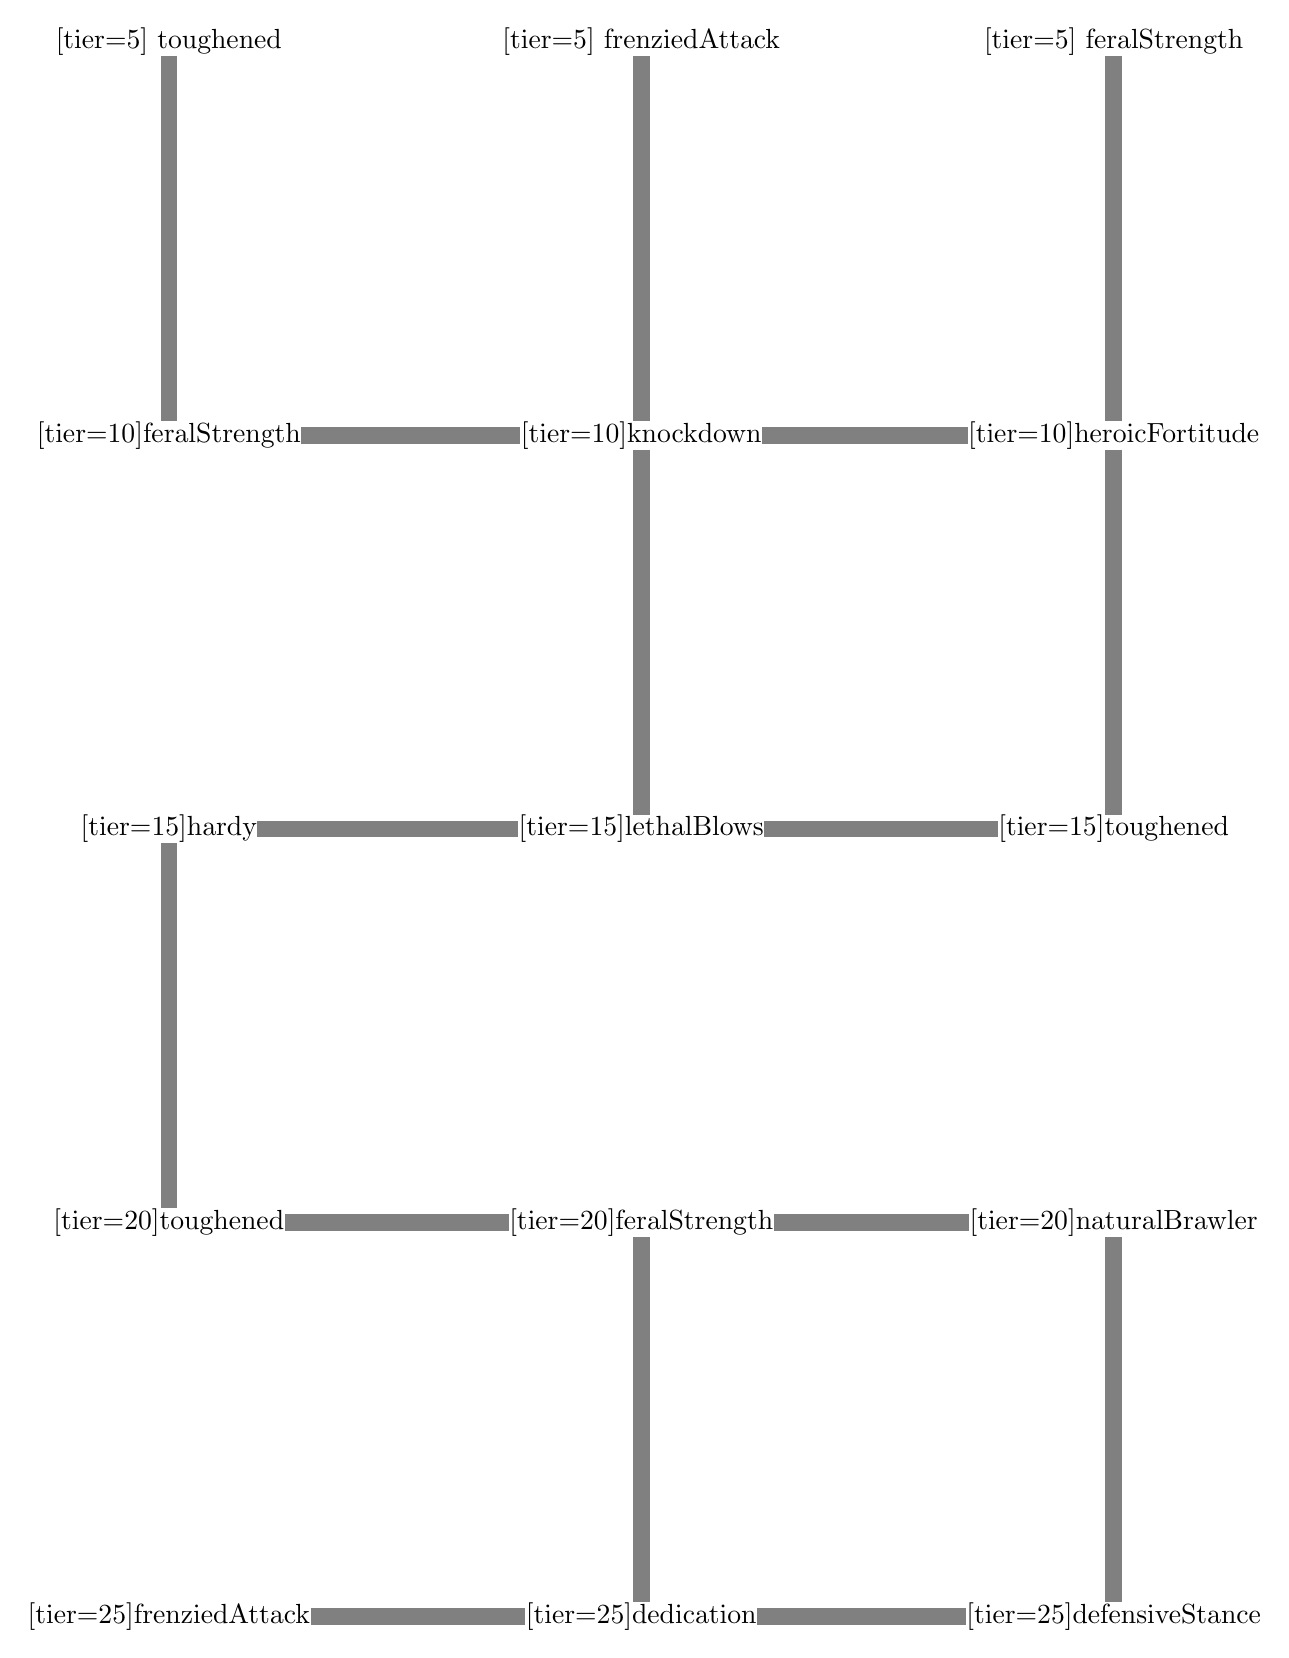
\begin{tikzpicture}
        \draw ( 0,  0) node(aa)[inner sep=0]{\TalentBox[tier=5] {toughened}}
              ( 6,  0) node(ab)[inner sep=0]{\TalentBox[tier=5] {frenziedAttack}}
              (12,  0) node(ac)[inner sep=0]{\TalentBox[tier=5] {feralStrength}}
              ( 0, -5) node(ba)[inner sep=0]{\TalentBox[tier=10]{feralStrength}}
              ( 6, -5) node(bb)[inner sep=0]{\TalentBox[tier=10]{knockdown}}
              (12, -5) node(bc)[inner sep=0]{\TalentBox[tier=10]{heroicFortitude}}
              ( 0,-10) node(ca)[inner sep=0]{\TalentBox[tier=15]{hardy}}
              ( 6,-10) node(cb)[inner sep=0]{\TalentBox[tier=15]{lethalBlows}}
              (12,-10) node(cc)[inner sep=0]{\TalentBox[tier=15]{toughened}}
              ( 0,-15) node(da)[inner sep=0]{\TalentBox[tier=20]{toughened}}
              ( 6,-15) node(db)[inner sep=0]{\TalentBox[tier=20]{feralStrength}}
              (12,-15) node(dc)[inner sep=0]{\TalentBox[tier=20]{naturalBrawler}}
              ( 0,-20) node(ea)[inner sep=0]{\TalentBox[tier=25]{frenziedAttack}}
              ( 6,-20) node(eb)[inner sep=0]{\TalentBox[tier=25]{dedication}}
              (12,-20) node(ec)[inner sep=0]{\TalentBox[tier=25]{defensiveStance}}
        ;

        \tikzstyle{bar}=[gray,-,>=stealth, line width=6pt]

        \draw [bar] (aa) to (ba);
        \draw [bar] (ab) to (bb);
        \draw [bar] (ac) to (bc);
        \draw [bar] (bb) to (cb);
        \draw [bar] (bc) to (cc);
        \draw [bar] (ca) to (da);
        \draw [bar] (db) to (eb);
        \draw [bar] (dc) to (ec);

        \draw [bar] (ba) to (bb);
        \draw [bar] (bc) to (bb);

        \draw [bar] (ca) to (cb);
        \draw [bar] (cc) to (cb);

        \draw [bar] (da) to (db);
        \draw [bar] (dc) to (db);

        \draw [bar] (ea) to (eb);
        \draw [bar] (ec) to (eb);

    \end{tikzpicture}
}
